\setchapterpreamble[u]{\margintoc}
\chapter{Վիճակագրական բնութագրիչներ}
\labch{descriptors}

\emergencystretch 2em

\section{Մաթսպասում}

Խաղում ենք հետևյալ խաղը։ Ամեն անգամ ընտրում ենք $1$-$38$ թվերից որևէ մեկը (ենթադրենք՝ $8$), կատարում ենք $\$1$-ի խաղադրույք, պտտում ռուլետկան և
\begin{itemize}
    \item եթե ընկնում է $8$, ապա շահում ենք $\$36$
    \item հակառակ դեպքում՝ կորցնում $\$1$-ը
\end{itemize}

\question{Կխաղայի՞ք արդյոք այսպիսի խաղ։}

Հավանաբար կպատասխանեք, որ ոչ, քանի որ հաղթելու հավանակա\-նու\-թյունը շատ փոքր է, իսկ շահելու ենթակա գումարը՝ ոչ այնքան մեծ։ 


\begin{marginfigure}
    \centering
    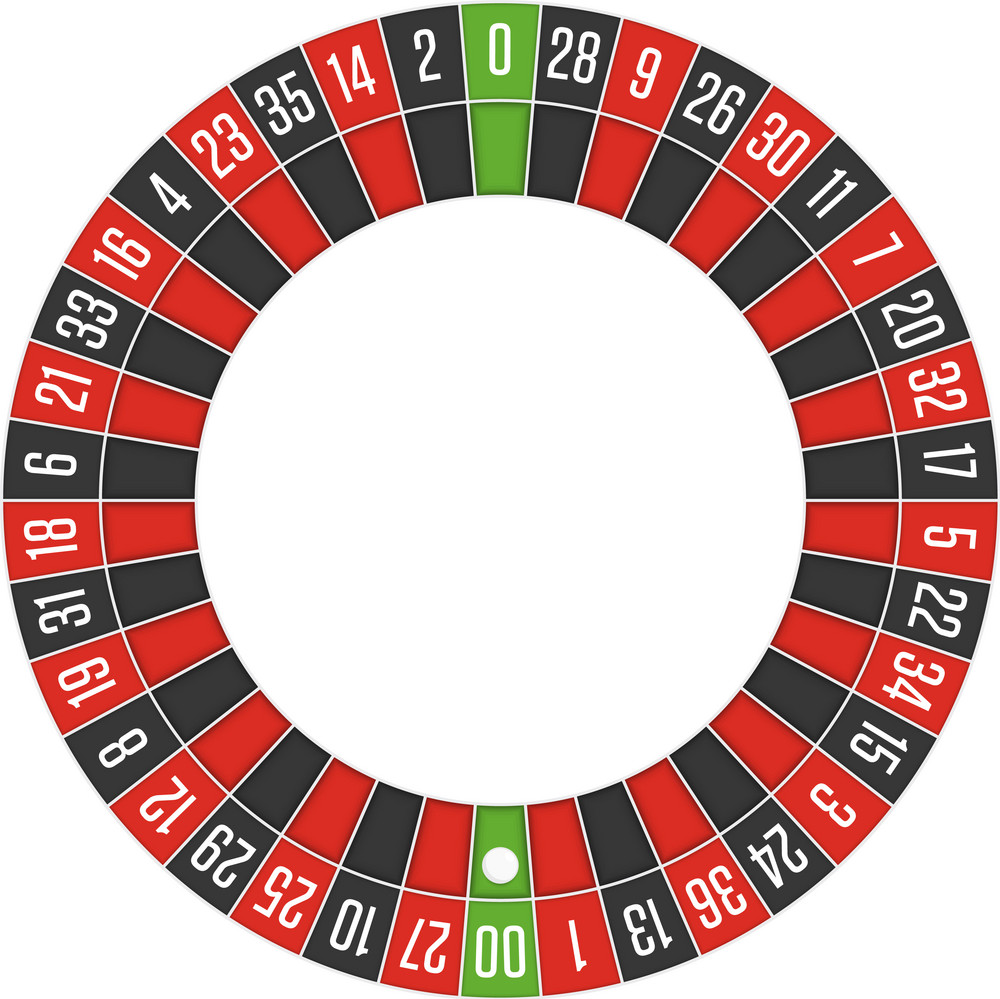
\includegraphics[width=0.8\linewidth]{chapters/chapter 10/roulette.png}
\end{marginfigure}

\question{Իսկ եթե $8$ ընկնելու դեպքում շահեիք $\$150$՞։ Իսկ $\$37.01$-ի դեպքո՞ւմ։}

Քանի որ հաղթելու հավանականությունն ընդամենը $\dfrac{1}{38}$ է, ապա կոպիտ ասած՝ եթե $38\,000$ անգամ պտտենք, $1000$ անգամը կընկնի մեր պահած թիվը, արդյունքում կշահենք
\[
1000 \cdot \color{mygreen}37.01
\]
իսկ մնացած անգամները՝ կկորցնենք
\[
37000 \cdot \color{myred}(-1)
\]
Ուրեմն ընդհանուր առմամբ $38\,000$ անգամ խաղալով կունենանք մոտ
\[
1000 \cdot 37.01 + 37000 \cdot (-1) = 10
\]
դոլարի շահույթ, կամ միջինում ամեն մի խաղում՝
\[
\frac{1000}{38000} \cdot 37.01 + \frac{37000}{38000} \cdot (-1) = \frac{10}{38000}
\]
այսինքն՝ $\approx \$0.0003$ շահույթ։ 

Այս թիվը իհարկե մեծ չէ, բայց դրական է․ եթե այս խաղը խաղանք մի քանի միլիարդ անգամ, կարող ենք միլիոնների շահույթ ակնկալել։ Բնականաբար, հնարավոր է՝ բախտներս չբերի, մեր սպասածից քիչ տանենք, կամ էլ հակառակը՝ բախտի բերմամբ հաջողվի շատ գումար տանել, բայց միջինում կարող ենք \textit{սպասել} ամեն խաղից մոտ $\approx \$0.0003$-ի շահույթ։ 

\begin{definition}
$X$ դիսկրետ պատահական մեծության \textbf{մաթսպա\-սում}\marginnote{անգլերեն՝ {\it expected value}} կանվանենք
\[
\E[X] =  \sum_{x_k} x_k\cdot \PP[X=x_k] 
\]
թիվը։
\end{definition}

Այսինքն՝ հերթով կդիտարկենք $X$ պատահական մեծության բոլոր հնա\-րավոր $x_k$ արժեքները և կվերցնենք դրանց \textit{կշռավորված միջինը՝}
\[
\E[X] = \sum_{X\text{-ի արժեքները}} \overbrace{x_k}^{\text{ամեն արժեք}}\cdot \underbrace{\PP[X=x_k]}_{\text{իր հավանականությամբ}}
\]
Մասնավորապես եթե $X$-ի բոլոր արժեքներն ունեն նույն հավանականու\-թյունը, $\E[X]$-ը կլինի այդ արժեքների միջին թվաբանականը, իսկ եթե օրինակ՝ արժեքներից մեկը $100$ անգամ ավելի հավանական է, քան մյուսը, ապա $\E[X]$-ը հաշվելիս այն կունենա $100$ անգամ ավելի մեծ կշիռ։

\question{Եթե նետենք մետաղադրամն ու գիր ընկնելու դեպքում վերցնենք $X=1$, ղուշի դեպքում՝ $X=0$, որքա՞ն կլինի $\E[X]$-ը։}

\begin{example}\label{die_rv}
Նետում ենք զառն ու $X$-ով նշանակում ընկած թիվը։ Այդ դեպքում $X$-ի մաթսպասումը կլինի՝
\[
\E[X] = \frac{1}{6} \cdot 1 + \frac{1}{6} \cdot 2 + \dots + \frac{1}{6} \cdot 6 = \frac{1+2+\dots+6}{6} = \frac{7}{2} %3.5
\]
այսինքն բոլոր արժեքների միջինը։ 
\end{example}

Իսկ եթե ուզեինք պարզել $X^2$ արտահայտության \marginnote{$X^2$-ն \hyperref[transformed_rv]{\color{OliveGreen} ևս} պատահական մեծություն է}միջինը, պարզապես կվերցնեինք $X$-ի արժեքների քառակուսիներն ու կրկին կբազմապատ\-կե\-ինք այդ արժեքների հավանականություններով՝
\[
\E[X^{\color{myred} 2}] = \frac{1}{6} \cdot 1^{\color{myred} 2} + \frac{1}{6} \cdot 2^{\color{myred} 2} + \dots + \frac{1}{6} \cdot 6^{\color{myred} 2} = \frac{1^{\color{myred} 2}+2^{\color{myred} 2}+\dots+6^{\color{myred} 2}}{6} = \frac{91}{6} %\approx 15.17
\]

\warning{Ինչպես տեսնում ենք, $\E[X^2] \ne \E[X]^2$:}

Նույնը նաև $X^3$-ի, $\dfrac{1}{X}$-ի, $\cos(X)$-ի և առհասարակ ցանկացած $g(X)$ տեսքի պատահական մեծության համար՝\marginnote{այս կանոնը \href{https://en.wikipedia.org/wiki/Law_of_the_unconscious_statistician#Etymology}{անվանում են} {\rm LOTUS}}
\[
\E[g(X)] =  \sum_{x_k} g(x_k)\cdot \PP[X=x_k] 
\]
Եկեք հիմա սահմանենք մաթսպասման գաղափարը անընդհատ պա\-տա\-հական մեծության համար։ Քանի որ անընդհատ $X$-ի դեպքում նրա ցանկացած արժեք ընդունելու հավանականությունը $0$ է, $\PP[X=x_k]$-ն փոխարինենք իր անընդհատ անալոգով՝ $f_X(x)$ խտությամբ, իսկ քանի որ միջակայքում ընկած բոլոր թվերը չենք կարող գումարել, $\sum$ գումարի նշանը փոխարինենք ինտեգրալով՝
\begin{align*}
\PP[X=x] &\mapsto f_X(x) \\
\sum_{X\text{-ի արժեքները}} &\mapsto \int_{a}^{b}
\end{align*}
որտեղ $(a, b)$-ն այն միջակայքն է, որին պատկանում են $X$-ի բոլոր հնարավոր արժեքները։ \marginnote{$(a, b)$-ն այն $x$-երն են, որտեղ $f_X(x) \ne 0$} 
Ցանկության դեպքում կարող ենք իհարկե ինտեգրել ոչ թե միայն $(a, b)$ միջակայքի, այլ ողջ առանցքի երկայնքով՝ $(-\infty, \infty)$, բայց քանի որ $(a, b)$-ից դուրս $f_X(x)$-ը զրո է, ապա դա նույնը կլինի, ինչ ինտեգրել $(a, b)$-ով։ Ուրեմն,

\begin{definition}
$X$ անընդհատ պատահական մեծության \textbf{մաթ\-սպա\-սում} կանվանենք
\[
\E[X] = \int_{-\infty}^{+\infty} x \cdot f_X(x) \, dx
\]
թիվը։
\end{definition}
Կրկին այն միջակայքերը, որոնցում խտության ֆունկցիան ավելի մեծ է, կունենան ավելի շատ կշիռ, քան ավելի ցածր խտությամբ միջա\-կայքերը։ 

\begin{example}\label{metro}
Գագիկն ամեն օր «Բարեկամությունից» դասի գնալիս չափում է, թե նախատեսվածից քանի րոպե ուշ կամ շուտ է շարժվում մետրոն։ Չափումների շնորհիվ նա պարզել է, որ այդ րոպեների տարբերությունը ցույց տվող պատահական մեծության {\rm PDF}-ն է՝
\[
f_X(x) = e^{-x^2}
\]

\begin{marginfigure}
    \centering
    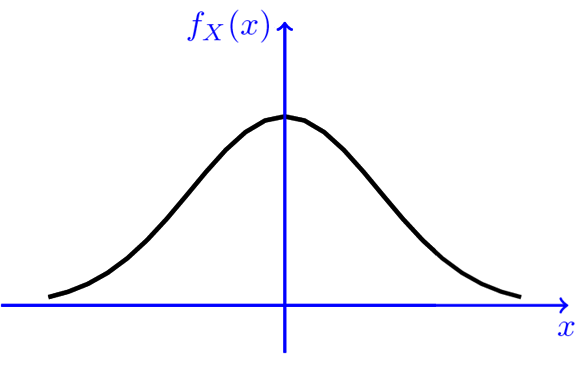
\includegraphics[width=\linewidth]{chapters/chapter 10/normal PDF.png}
    \caption*{$x$-երի առանցքը րոպեներն են}
\end{marginfigure}

Սկզբում փորձեք $f_X$-ի գրաֆիկին նայելով կռահել, թե միջինում քանի՞ րոպե է ուշանում մետրոն, ապա այն ճշգրիտ կհաշվենք։ 

Գրենք $\E[X]$-ը հետևյալ տեսքով և ինտեգրենք՝
\begin{align*}
\E[X]
= \int_{-\infty}^{+\infty} xe^{-x^2}\, dx
&= \frac{1}{2}\int_{-\infty}^{+\infty} e^{-x^2}(x^2)'\, dx \\
&= \frac{1}{2}\int_{-\infty}^{+\infty} e^{-x^2} d(x^2)
= \frac{1}{2} \left.e^{-x^2}\right|_{x=-\infty}^{+\infty} = 0
\end{align*}
Ուրեմն թեև որոշ օրերի մետրոն շուտ է շարժվում, որոշ օրերի՝ ուշ, միջինում այն շարժվում է․․․ ճիշտ ժամանակին։
\end{example}

Նման ձևով կարող ենք նաև $X$-ը դնել ցանկացած $g$ անընդհատ ֆունկցիայի մեջ և հաշվել $g(X)$-ի մաթսպասումը՝
\[
\E[g(X)] = \int_{-\infty}^{+\infty} g(x) \cdot f_X(x) \, dx
\]
\question{$X$-ը ի՞նչ ֆունկցիայի մեջ պետք է դներ Գագիկը, որպեսզի $\E[g(X)]$-ը ցույց տար միջինում մետրոյի շեղումը ժամացուցակից։}

Ենթադրենք հայտնի է, որ միջինում ամեն մեծահասակ մարդու համար ծախսվում է օրական $2500$ դրամ, իսկ ամեն երեխայի համար՝ $4000$ դրամ։

\question{Օրական միջինում որքա՞ն է ծախսում $1$ մեծից և $1$ երեխայից կազմված ընտանիքը։ Իսկ $2$ մեծից և $3$ երեխայի՞ց։}

Ինչպես տրամաբանորեն պետք է լիներ, \marginnote[*+3]{ավելի ընդհանուր՝ \[\E[X_1+X_2+\dots] = \E[X_1] + \E[X_2] + \dots\]}
\begin{align*}
\E[c \cdot X] &= c \cdot \E[X] \\
\E[X + c] &= \E[X] + c \\
\E[X + Y] &= \E[X] + \E[Y]
\end{align*}
և եթե մի պատահական մեծություն միշտ փոքր/հավասար է մյուսից՝ $X \le Y$, ապա $\E[X] \le \E[Y]$:

Իսկ ի՞նչ կարելի է ասել պատահական մեծությունների \textit{արտադրյալի} մաթսպասման մասին։ Պարզվում է, որ
\begin{theorem}\label{independence_E}
Եթե $X$-ն ու $Y$-ն անկախ են, ապա
\[
\E[X \cdot Y] = \E[X] \cdot \E[Y]
\]
\end{theorem}

\warning{Հակառակը ոչ միշտ է ճիշտ․ եթե $\E[XY] = \E[X] \cdot \E[Y]$, դա դեռ չի նշանակում, որ $X$-ն ու $Y$-ն անկախ են։}


\section{Վարիացիա}

Նկարում պատկերված են երկու տարբեր ընկերություններում աշխա\-տա\-վարձերի խտության գրաֆիկները:\marginnote{$=$ պատահական վերցված աշխատակցի աշխատավարձի {\rm PDF}-ը} Ինչպես տեսնում ենք, երկուսում էլ միջին աշխատավարձը $200\,000$ դրամ է, սակայն 
\begin{itemize}
    \item հիմնարկներից մեկում աշխատավարձերը մոտ են իրենց միջինին
    \item մյուսում՝ միջինից բավական հեռու են, ցրված են
\end{itemize}

\begin{figure}[b]
    \centering
    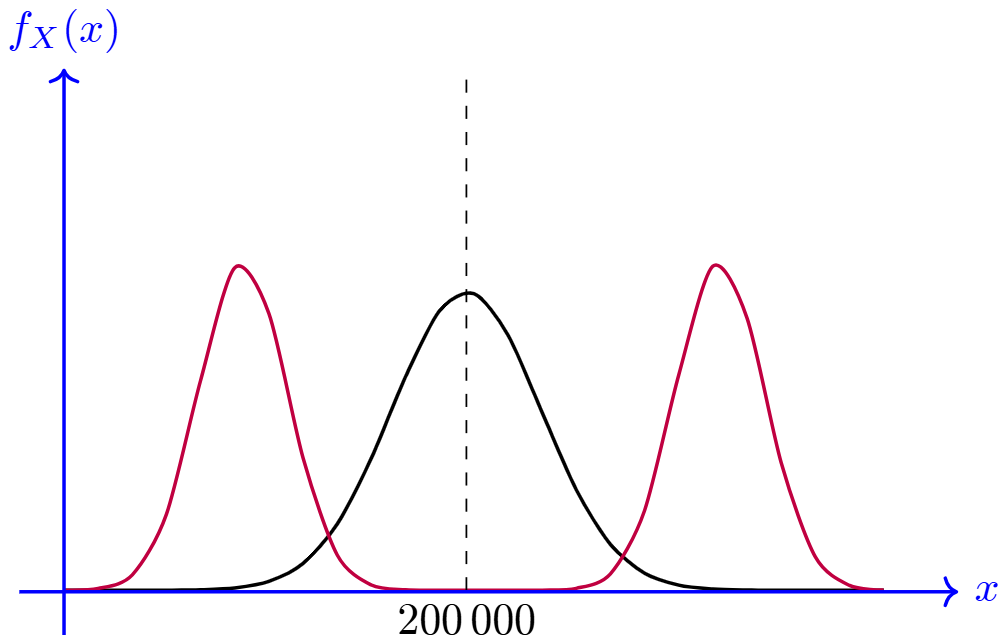
\includegraphics[width=0.65\linewidth]{chapters/chapter 10/salaries.png}
\end{figure}


% \begin{tikzpicture}[scale=1.2]
%   \draw[domain=0:5.5, smooth, variable=\x, thick]
%     plot ({\x}, {2*exp(-((\x - 2.7)^2)/(2*0.5^2))});

%   \draw[domain=0:5.5, smooth, variable=\x, thick, purple]
%     plot ({\x}, {
%       2.2*exp(-((\x - 1.2)^2)/(2*0.3^2)) +
%       2.2*exp(-((\x - 4.4)^2)/(2*0.3^2))
%     });
  
%   \draw[dashed] (2.7,0) -- (2.7,3.5);
%   \node[below] at (2.7,0) {$200\,000$};
%   \draw[->, thick, blue] (-0.3,-0.01) -- (6,-0.01) node[anchor=west] {\textcolor{blue}{$x$}};
%   \draw[->, thick, blue] (0,-0.3) -- (0,3.5) node[anchor=south] {\textcolor{blue}{$f_X(x)$}};
% \end{tikzpicture}

Ինչպե՞ս չափենք միջինից ունեցած այս շեղումը՝ $X$-ի արժեքների և $\E[X]$-ի հեռավորությունը։ Սկզբի համար կարող ենք յուրաքանչյուր աշխատակցի $X$ աշխատավարձից հանել այդ միջինը՝
\[
X - \E[X]
\]
Երկրաչափորեն սա կնշանակի $f_X$-ի գրաֆիկը $\E[X]$-ով տանել ձախ, այսինքն այնպես, որ ստացվածի միջինը լինի $0$։

Այն աշխատակիցների համար, որոնք ստանում էին միջինից բարձր աշխատավարձ՝ $X > \E[X]$, այս մեծությունը կլինի դրական, մյուսների համար՝ բացասական։ Թեև մեզ հարկավոր է այդ շեղումների միջինը, բայց եթե վերցնենք ստացվածի մաթսպասումը՝
\[
\E[X - \E[X]]
\]
շատ ստացողների դրական շեղումը կկրճատվի քիչ ստացողների բա\-ցա\-սական շեղման հետ, և հնարավոր է՝ ստանանք $0$, ինչպես \hyperref[metro]{\color{OliveGreen} մետրոյի} օրինակում։ Ուրեմն դարձնենք այս տարբերությունը դրական։

Տարբերակներից մեկն է վերցնել ստացվածի մոդուլը, ապա հաշվել դրա միջինը՝
\[
\E\left[\left|X - \E[X]\right|\right]
\]
մեկ ուրիշ տարբերակ է մոդուլի փոխարեն բարձրացնել քառակուսի՝
\[
\E\left[\left(X - \E[X]\right)^2\right]
\]

\question{Ո՞րը կընտրեիք Դուք։ Ո՞րը երբ պետք կգա։}

\begin{example}
Ենթադրենք $X$-ը ինչ-որ պատահական մեծություն է, որն ընդունում է երեք արժեք՝ $0$, $10$ և $15$, հետևյալ հավանականություն\-նե\-րով՝
\[
\PP[X = 0] = 0.6, \qquad \PP[X = 10] = \PP[X = 15] = 0.2
\]
Անշուշտ, $X$-ի արժեքներն իրենց միջինից՝
\[
\E[X] = 0 \cdot 0.6 + 10 \cdot 0.2 + 15 \cdot 0.2 = 5
\]
բավականին շեղված են։ Շեղման չափը՝ $X-\E[X]$-ը, $0.6$ հավանակա\-նու\-թյամբ հավասար է $-5$, $0.2$-ով՝ $5$, $0.2$-ով՝ $15$, հետևաբար\marginnote[*+1]{ինքնուրույն ստուգեք սա}
\[
\E\left[\left|X - \E[X]\right|\right]
= 
0.6 \cdot |-5| + 0.2 \cdot |5| + 0.2 \cdot |15|
=
7
\]
իսկ 
\[
\E\left[\left(X - \E[X]\right)^2\right]
=
0.6 \cdot (-5)^2 + 0.2 \cdot 5^2 + 0.2 \cdot 15^2
= 
65
\]
Այժմ $X$-ի արժեքներից մեկը $1$ միավորով մոտեցնենք միջինին, մյուսը՝ նույնքան հեռացնենք, և ստացվածը նշանակենք $Y$-ով․
\[
\PP[Y = 0] = 0.6, \qquad \PP[Y = 9] = \PP[Y = 16] = 0.2
\]
Այս գործողությունը անելիս մաթսպասումը չի փոխվի՝ $\E[Y]=\E[X]=5$, իսկ արժեքների հեռավորությունները $\E[Y]$-ից
\begin{itemize}
\item մոդուլով հաշվելու դեպքում կմնա նույնը․
\[
\E\left[\left|Y - \E[Y]\right|\right]
=
0.6 \cdot |-5| + 0.2 \cdot |4| + 0.2 \cdot |16|
= 
1
\]
\item քառակուսիով հաշվելու դեպքում՝ կմեծանա․
\[
\E\left[\left(Y - \E[Y]\right)^2\right]
=
0.6 \cdot (-5)^2 + 0.2 \cdot 4^2 + 0.2 \cdot 16^2
= 
69.4
\]
\end{itemize}

Եթե արժեքները ևս $1$-ով բրդենք համապատասխանաբար ձախ ու աջ՝
\[
\PP[Z = 0] = 0.6, \qquad \PP[Y = 8] = \PP[Y = 17] = 0.2
\]
մաթսպասումն ու մոդուլով հեռավորությունը նորից կմնան նույնը, իսկ քառակուսիովը՝ կրկին կմեծանա․
\[
\E\left[\left(Z - \E[Z]\right)^2\right]
=
0.6 \cdot (-5)^2 + 0.2 \cdot 3^2 + 0.2 \cdot 17^2
= 
74.6
\] 
և այդպես շարունակ․ չնայած մեր պատահական մեծության որոշ ար\-ժեք\-ներ ավելի ու ավելի են հեռանում միջինից, մոդուլով հեռա\-վո\-րու\-թյունն այդ ցրվածությունը չի ֆիքսում, իսկ քառակուսով հե\-ռա\-վո\-րու\-թյունը՝ գնալով ավելի մեծ թվեր է վերադարձնում։
\end{example}

Պատճառն, իհարկե, քառակուսին է․ որքան մեծ է ինչ-որ արժեքի շեղումը, այնքան ավելի մեծ է նրա քառակուսին։ Ավելի պատկերավոր օրինակ՝

\begin{example}
Ձեզ պետք է արյան ճնշումը $10$ մմ ս․ս․-ով բարձրացնել։ Դեղատանն առաջարկում են երկու դեղ՝
\begin{itemize}
\item մեկը խմելիս ճնշումը կբարձրանա $X$-ով, ընդ որում
\[
\hspace{-2em}\PP[X=8.75] = 0.6, \qquad \PP[X=10.5] = 0.3, \qquad \PP[X=16] = 0.1
\]
\item մյուսի դեպքում՝ $Y$-ով, ընդ որում
\[
\hspace{-2em}\PP[Y=6.8] = 0.25, \qquad \PP[Y=10] = 0.7, \qquad \PP[Y=26] = 0.05
\]
\end{itemize}
Ո՞ր դեղը կնախընտրեք խմել։
Եթե վաճառողին հարցնեք, թե ո՞րն է ավելի վստահելի, նա կպատասխանի, որ երկու դեղերն էլ նույնն են՝ միջինում ազդեցությունը $10$ է, մոդուլով միջին շեղման չափը՝ $1.6$։ 

Մինչդեռ եթե հարցնեք դրանց միջին քառակուսային շեղումները՝\marginnote{ավելի ճշգրիտ՝ շեղման քառակուսիները}
\begin{align*}
\E\left[\left(X - \E[X]\right)^2\right] &= 1.25^2 \cdot 0.6 + 0.5^2 \cdot 0.3 + 6^2 \cdot 0.1 \approx 4.6\\
\E\left[\left(Y - \E[Y]\right)^2\right] &= 3.2^2 \cdot 0.25 + 0^2 \cdot 0.7 + 16^2 \cdot 0.05 \approx 15.4
\end{align*}
կտեսնեք, որ երկրորդի շեղումն անհամեմատ ավելի մեծ է, այսինքն՝ երկրորդն ավելի \textit{ռիսկային} է։
\end{example}

Իրոք, այն փաստը, որ $5\%$ հավանականություն կա, որ արյան ճնշումը $10$-ի փոխարեն $26$-ով կբարձրանա, որևէ ձևով չի արտացոլվում մոդուլով շեղման մեջ, իսկ քառակուսիով հաշվելիս զգացվում է։ Հետևաբար երկրորդ տարբերակով շեղման չափը հաշվելն ավելի պիտանի է ռիսկերը գնահատելու տեսանկյունից։ 

\begin{definition}
$X$ պատահական մեծության ցրվածք կամ \textbf{վարիացիա} կանվանենք\marginnote{անգլերեն՝ {\it variance}} 
\[
\Var[X] = \E\left[\left(X - \E[X]\right)^2\right] 
\]
թիվը, իսկ դրա արմատը կանվանենք \marginnote{{\it standard deviation}}\textbf{ստանդարտ շեղում:}
\end{definition}

Ինչպես տեսանք վերևում և ինչպես երևում է բանաձևից, վարիացիան ցույց է տալիս, թե միջինում պատահական մեծության արժեքները որքանով են հեռու իրենց միջինից։ Քանի որ այդ հեռավորությունը \marginnote{ինչ-որ իմաստով՝ $\Var[X]$-ը $X$-ի ու $\E[X]$-ի $\operatorname{L}_2$ հեռավորության քառա\-կու\-սին է ($\approx$ $X$-ի նորմի քառակուսին)} հաշվելիս շեղումները քառակուսի ենք բարձրանում, ապա նոր «միջի\-նաց\-նում», իմաստ ունի ստացված թվի արմատը դիտարկելը․ այդտեղից էլ ստանդարտ շեղման օգտակարությունը։

\warning{Ինչպես $\E[X]$-ը, այդպես էլ $\Var[X]$-ը թվեր են, ոչ թե պատահական մեծություններ։}

Քանի որ այնքան էլ հարմար չէ այս բանաձևով $\Var[X]$-ը հաշվել, փորձենք այն պարզեցնել․\marginnote[*+2]{հաստատունները նշված են {\color{myblue} կապույտով}}
\begin{align*}
\Var[X] 
&= \E\left[\left(X - {\color{myblue}\E[X]}\right)^2\right] 
= \E\left[X^2 - {\color{myblue} 2} \cdot X \cdot {\color{myblue}\E[X]} + {\color{myblue}\E[X]^2} \right] 
\\
&= \E\left[X^2\right] - \E\left[{\color{myblue} 2} \cdot X \cdot {\color{myblue}\E[X]}\right] + {\color{myblue}\E[X]}^2
\\
&= \E\left[X^2\right] - {\color{myblue} 2} \cdot {\color{myblue}\E[X]} \cdot \E\left[X \right] + {\color{myblue}\E[X]}^2 = \E\left[X^2\right] - \E[X]^2
\end{align*}
Ստացանք բավականին հարմար բանաձև՝ $\Var[X] = \E[X^2] - \E[X]^2$:

\begin{example}
\hyperref[die_rv]{\color{OliveGreen} Կրկին} $X$-ով նշանակենք զառը նետելիս ընկնող թիվը։ Այդ թվի վարիացիան կլինի՝
\[
\Var[X] = \E[X^2] - \E[X]^2 = \frac{91}{6} - \left(\frac{7}{2}\right)^2 \approx 2.92
\]
իսկ ստանդարտ շեղումը՝ $\approx 1.71$:
\end{example}

Մինչև առաջ անցնելը նկատենք վարիացիայի մի քանի հատկություններ։ Նախ՝ հեռավորության քառակուսին չի կարող լինել բացասական, ուրեմն
\[
\Var[X] \ge 0
\]
ընդ որում՝ զրոյի հավասար կարող է լինել միայն եթե $X$-ի բոլոր արժեքները նույնն են, այսինքն $X$-ն ընդունում է միայն մեկ արժեք։ 

Ի տարբերություն մաթսպասման՝ երբ պատահական մեծությունը բազմապատկում ենք որևէ թվով, նրա վարիացիան բազմապատկվում է այդ թվի քառակուսիով՝
\[
\Var[c\cdot X] = c^2 \cdot \Var[X]
\]
իսկ արժեքները հաստատունով մեծացնելիս կամ փոքրացնելիս դրանց ցրվածությունը, բնականաբար, չի փոխվում՝
\[
\Var[X + c] = \Var[X]
\]

\warning{Շատ դեպքերում $\Var[X + Y] \ne \Var[X] + \Var[Y]$:}
\question{Ի՞նչ եք կարծում, ե՞րբ կլինի $\Var[X+Y] = \Var[X] + \Var[Y]$:}

Իրոք, սահմանման մեջ առկա քառակուսու պատճառով
\[ 
\Var[X + Y] = \Var[X] + \Var[Y] + 2\left(\E[XY] - \E[X] \cdot \E[Y]\right)
\]
այսինքն՝ \marginnote{ինչպես \textit{ուղղահայաց} $\va$ ու $\vb$-ի դեպքում \[\|\va+\vb\|^2 = \|\va\|^2 + \|\vb\|^2\] այնպես էլ \textit{անկախ} $X$ ու $Y$-ի դեպքում՝ \[\Var[X+Y] = \Var[X] + \Var[Y]\]} գումարի վարիացիան կախված է ոչ միայն առանձին-առանձին գումարելիների վարիացիաներից, այլև դրանց՝ \textit{իրար հետ ունեցած} կապից։
Իսկ երբ $X$-ն ու $Y$-ն անկախ են, $\E[XY]$-ը \hyperref[independence_E]{\color{OliveGreen} հավասար է լինում} $\E[X] \cdot \E[Y]$-ի, և ունենում ենք $\Var[X] + \Var[Y]$։

\section{Կովարիացիա}

Ենթադրենք ունենք երկու պատահական մեծություններ, ասենք՝ «Տեսլա» և «Երազ» ընկերությունների արժեթղթերը։ \marginnote{այսինքն՝ պատահական վերցված օրը որքա՞ն են դրանց արժեքները} Ինչպե՞ս պարզենք, թե որքա\-նով են դրանք իրարից կախված, կամ ավելի կոնկրետ՝ երբ դրան\-ցից մեկը աճում/նվազում է, որքան է փոխվում մյուսը։ 

\begin{figure}[h]
    \centering
    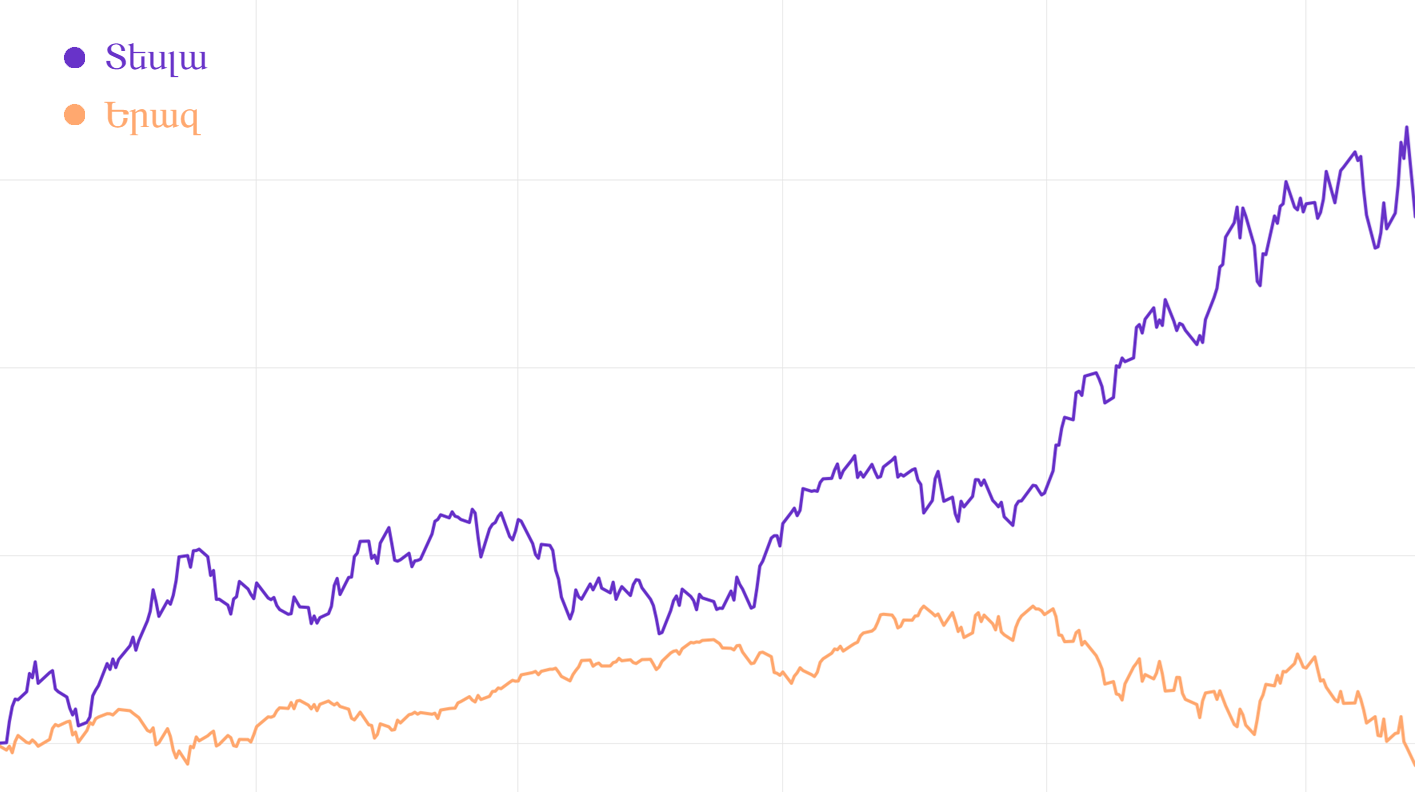
\includegraphics[width=0.65\linewidth]{chapters/chapter 10/stocks.png}
\end{figure}

\question{Ի՞նչ գործիք էինք օգտագործում երկու $\va$ և $\vb$ վեկտորների կապը/նմանությունը չափելու համար։}

Նախ կարող ենք $xy$-հարթության վրա պատկերել $X$-ի և $Y$-ի միաժամանակ ունեցած արժեքների թվազույգերը, տվյալ դեպքում՝ ամեն օրվա համար նշել $(x, y)$ կետը, որտեղ $x$-ն այդ օրը «Տեսլայի» արժեթղթի գինն է, $y$-ը՝ «Երազի»։ 

Խելքին մոտ կլինի նաև, եթե $X$ պատահական մեծության փոփոխության չափ ասելով հասկանանք նրա արժեքների՝ իր միջինի համեմատ ունեցած տարբերությունը՝ $X - \E[X]$, և ներմուծենք մի այսպիսի գործիք․

\begin{definition}
$X$ և $Y$ պատահական մեծությունների \textbf{կովարիա\-ցիա} կանվանենք
\[
\Cov[X, Y] = \E\left[(X-\E[X])(Y-\E[Y])\right]
\]
թիվը։
\end{definition}

Փաստորեն կովարիացիան ցույց է տալիս, թե միջինում որքան է $X$-ի փոփոխության և $Y$-ի փոփոխության արտադրյալը։ Եթե օրինակ՝ $X$-ը (իր միջինի համեմատ) $1$ միավորով\marginnote{գծային հանրահաշվի լեզվով ասած՝ կովարիացիան պատահական մեծու\-թյուն\-ների սկալյար արտադրյալն է} մեծանալիս $Y$-ը (իր միջինի համեմատ) միշտ մեծանա $5$ միավորով, իսկ $X$-ը $1$-ով փոքրանալիս էլ՝ փոքրանա $5$-ով, ապա կունենանք $\Cov[X, Y] = 5$։ 

\newpage

\begin{figure}[t]
\centering %
\floatsetup{floatrowsep=qquad}
\begin{floatrow}[3]%
\ffigbox[\FBwidth]{\caption*{\centering $\Cov[X, Y] > 0$}}{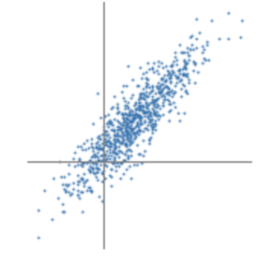
\includegraphics[width=0.4\textwidth]{chapters/chapter 10/covariance 1.png}}
\ffigbox[\FBwidth]{\caption*{\centering $\Cov[X, Y] < 0$}}{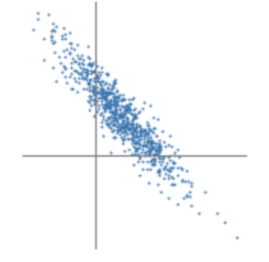
\includegraphics[width=0.4\textwidth]{chapters/chapter 10/covariance 2.png}}
\ffigbox[\FBwidth]{\caption*{\centering $\Cov[X, Y]$-ը մոդուլով փոքր է}}{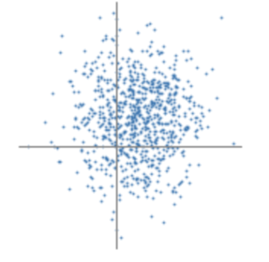
\includegraphics[width=0.4\textwidth]{chapters/chapter 10/covariance 3.png}}
\end{floatrow}
\end{figure}

Սա նշանակում է, որ $\Cov[X, Y]$-ը ցույց է տալիս $X$-ի ու $Y$-ի միջև եղած \textit{գծային կախումը՝} թե միջինում մեկի գծային աճը որքան փոփոխության է հանգեցնում մյուսի արժեքում (և հակառակը)։ Ստացված թիվը համաչափ է՝
\[
\Cov[X, Y] = \Cov[Y, X]
\]

\begin{example}
Նետենք $3$ մետաղադրամ, $X$-ով նշանակենք գիր ընկածների թիվը, $Y$-ով՝ ղուշ ընկածներինը։ Փորձենք հաշվել $\Cov[X, Y]$-ը։

Նախ, ի՞նչ հնարավոր արժեքներ կարող են ընդունել $X$-ն ու $Y$-ը միաժամանակ՝
\begin{itemize}
    \item $X=0$, $Y=3$
    \item կամ $X=1$, $Y=2$
    \item կամ $X=2$, $Y=1$
    \item կամ էլ $X=3$, $Y=0$
\end{itemize}
Որքա՞ն է, ասենք, $X=1$ և $Y=2$ լինելու հավանականությունը․\marginnote{արդյո՞ք $X$-ն ու $Y$-ն անկախ են}
\[
\PP[(X = 1) \text{ և } (Y = 2)] =\ ?
\]
Կարող ենք այս պատահույթը բաժանել երեք ենթադեպքի՝
\begin{itemize}
    \item առաջինը գիր, մյուս երկուսը ղուշ՝ ԳՂՂ
    \item երկրորդը գիր, մյուս երկուսը ղուշ՝ ՂԳՂ
    \item երրորդը գիր, մյուս երկուսը ղուշ՝ ՂՂԳ
\end{itemize}
Սրանցից յուրաքանչյուրի հավանականությունը
\[
\PP[\text{ԳՂՂ}] = 
\PP[\text{ՂԳՂ}] = 
\PP[\text{ՂՂԳ}] = 
\frac{1}{2} \cdot \frac{1}{2} \cdot \frac{1}{2} = \frac{1}{8}
\]
է, հետևաբար
\[
\PP[(X = 1) \text{ և } (Y = 2)] = 3 \cdot \frac{1}{8} = \frac{3}{8}
\]
և ճիշտ նույն ձևով\marginnote{վերևում գրվածի մեջ փոխենք «գիր» և «ղուշ» բառերի տեղերը} $\PP[(X = 2) \text{ և } (Y = 1)] = \dfrac{3}{8}$։

\newpage

Նման եղանակով հաշվելով մյուս երկու դեպքերի հավանականություն\-ները՝ կունենանք այսպիսի պատկեր․
\begin{center}
  \begin{tabular}{|c|c|c|}
    \hline
    $X$ & $Y$ & \textbf{հավանականություն} \\
    \hline
    $0$ & $3$ & $1/8$ \\
    \hline
    $1$ & $2$ & $3/8$ \\
    \hline
    $2$ & $1$ & $3/8$ \\
    \hline
    $3$ & $0$ & $1/8$ \\
    \hline
  \end{tabular}
\end{center}
Այժմ հաշվենք $X$-ի ու $Y$-ի մաթսպասումները՝
\[
\E[X] = 
0 \cdot \frac{1}{8} +
1 \cdot \frac{3}{8} +
2 \cdot \frac{3}{8} +
3 \cdot \frac{1}{8} =
1.5 = \E[Y]
\]
և հանենք դրանք յուրաքանչյուր տողում գրված արժեքներից․
\begin{center}
  \begin{tabular}{|c|c|c|}
    \hline
    $X - \E[X]$ & $Y - \E[Y]$ & \textbf{հավանականություն} \\
    \hline
    $-1.5$ & $1.5$ & $1/8$ \\
    \hline
    $-0.5$ & $0.5$ & $3/8$ \\
    \hline
    $0.5$ & $-0.5$ & $3/8$ \\
    \hline
    $1.5$ & $-1.5$ & $1/8$ \\
    \hline
  \end{tabular}
\end{center}
Կունենանք, որ 
\begin{align*}
\PP\big[(X - \E[X])(Y - \E[Y]) = -2.25\big] &= \frac{2}{8}\\
\PP\big[(X - \E[X])(Y - \E[Y]) = -0.25\big] &= \frac{6}{8}
\end{align*}
հետևաբար $X$-ի ու $Y$-ի կովարիացիան կլինի 
\[
\E\left[(X - \E[X])(Y - \E[Y])\right]
= -2.25 \cdot \frac{2}{8} + (-0.25) \cdot \frac{6}{8}
= -\frac{3}{4} = -0.75
\]
Ստացվեց բացասական կովարիացիա․ իրոք, ըստ սահմանման՝ երբ $X$-ը աճում է, $Y$-ը պիտի նվազի։
\end{example}

\question{Իսկ որքա՞ն է $\Cov[X, X+Y]$-ը (առանց հաշվելու)։}

Ինչպես կարող եք ենթադրել, եթե երկու պատահական մեծություններ իրարից անկախ են, նրանց կովարիացիան $0$ է՝\marginnote[*+2]{$X-\E[X]$-ն ու $Y-\E[Y]$-ն անկախ են}
\begin{align*}
\Cov[X, Y] &= \E\left[(X - \E[X])(Y - \E[Y])\right]
\\&= \E\left[X - \E[X]\right] \cdot \E\left[Y - \E[Y]\right]
= (\E[X] - \E[X]) \cdot (\E[Y] - \E[Y]) = 0
\end{align*}
բայց հակառակը ոչ միշտ է ճիշտ։ Թեկուզ միայն այն պատճառով, որ

\warning{Կովարիացիան ցույց է տալիս միայն պատահական մեծությունների միջև եղած \textbf{գծային} կապը։}

Այսինքն՝ հնարավոր է, որ պատահական մեծությունները իրար հետ կապված լինեն (ոչ թե գծային, այլ ասենք՝ քառակուսային կապով), բայց կովարիացիան դա չկարողանա «տեսնել»։

\newpage

\begin{example}
Ենթադրենք $X$ պատահական մեծությունն ընդունում է երեք արժեք՝
\[
\PP[X = -1] = \PP[X = 0] = \PP[X = 1] = \frac{1}{3}
\]
իսկ $Y$-ը նրա քառակուսին է՝ $Y = X^2$։ \marginnote{կարո՞ղ եք ինքնուրույն շարունակել} Բնականաբար $X$-ն ու $Y$-ն անկախ չեն, սակայն
\[
\E[X] = 0, \qquad \E[Y] = \frac{2}{3}
\]

\begin{marginfigure}
    \centering
    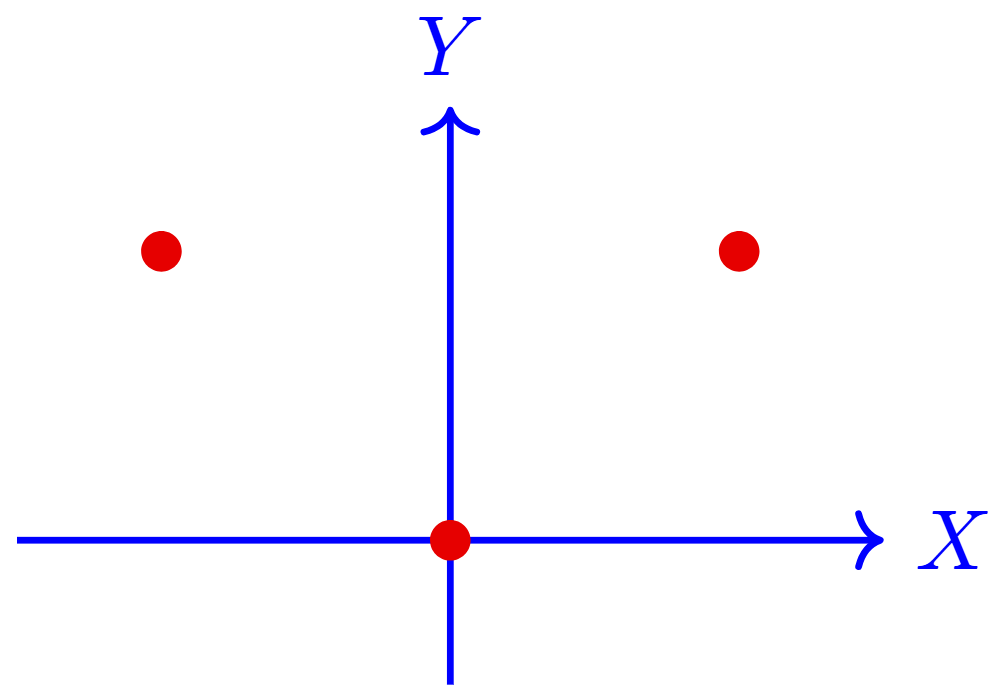
\includegraphics[width=0.8\linewidth]{chapters/chapter 10/three points.png}
\end{marginfigure}

% \begin{tikzpicture}[scale=1.2]
%   \draw[->, thick, blue] (-1.5,0) -- (1.5,0) node[anchor=west] {\textcolor{blue}{$X$}};
%   \draw[->, thick, blue] (0,-0.5) -- (0,1.5) node[anchor=south] {\textcolor{blue}{$Y$}};
%   \fill[myred] (-1,1) circle (2pt);
%   \fill[myred] (0,0) circle (2pt);
%   \fill[myred] (1,1) circle (2pt);
% \end{tikzpicture}

և հնարավոր արժեքների հավանականություններն են․
\begin{center}
  \begin{tabular}{|c|c|c|}
    \hline
    $X$ & $Y$ & \textbf{հավանականություն} \\
    \hline
    $-1$ & $1$ & $1/3$ \\
    \hline
    $0$ & $0$ & $1/3$ \\
    \hline
    $1$ & $-1$ & $1/3$ \\
    \hline
  \end{tabular}
\end{center}
որտեղից ստանում ենք՝
\[
\Cov[X, Y] = 
(-1) \cdot \frac{2}{3} \cdot \frac{1}{3} +
0 \cdot 0 \cdot \frac{1}{3} +
1 \cdot \frac{2}{3} \cdot \frac{1}{3} = 0
\]
Իրոք, թեև $X$-ն ու $Y$-ն անկախ չեն, բայց $X$-ի և՛ մեծանալիս, և՛ փոքրանալիս $Y$-ը փոխվում է նույն ձև՝ մեծանում է, այսինքն դրանց միջև եղած կապը գծային չէ՝ $\Cov[X, Y] = 0$:
\end{example}

Այնուամենայնիվ, կովարիացիան շատ օգտակար գործիք է երկու մեծությունների հնարավոր կապը բացահայտելու համար։ Վերևում արված երկար ու ձանձրալի հաշվարկներից խուսափելու համար կովարիացիայի սահմանման մեջ բացենք փակագծերն ու պարզեցնենք․ կստանանք՝
\[
\Cov[X, Y] = \E[XY] - \E[X] \cdot \E[Y]
\]
որտեղից կունենանք մեզ հետաքրքրող մյուս հատկությունները՝
\begin{align*}
\Cov[c \cdot X, Y] &= \Cov[X, c \cdot Y] = c \cdot \Cov[X, Y] \\
\Cov[X, Y_1 + Y_2] &= \Cov[X, Y_1] + \Cov[X, Y_2]
\end{align*}
իսկ մասնավորապես դրանցից երկրորդի շնորհիվ՝ ոչ այնքան հետաքրքիր հաջորդ հատկությունը․
\begin{align*}
\Cov[X_1 + X_2, Y_1 + Y_2]&= \Cov[X_1, Y_1] + \Cov[X_1, Y_2] \\&+ \Cov[X_2, Y_1] + \Cov[X_2, Y_2]
\end{align*}
որը կասկածելիորեն նման է բազմապատկելիս փակագծերը բացելուն՝ $(a+b)(c+d) = \dots$: 

\question{Ի՞նչ կստացվի, եթե $Y$-ի փոխարեն տեղադրենք $X$։ Ինչպե՞ս կմեկնաբանեք ստացվածը։}

Բնականաբար, եթե պատահական մեծություններից մեկը \marginnote[*+1]{$=$ ընդունում է միայն մեկ արժեք} հաստատուն է՝ $Y=c$, ապա $\Cov[X, Y] = 0$։


\section{Կոռելացիա}

\textit{— Բայց մի րոպե,— կարող եք հարցնել,— ի՞նչ է նշանակում $\Cov[X, Y] = 60$․ վերջը կա՞ գծային կապ, թե՞ ոչ։}

Իհարկե, եթե կովարիացիան դրական է, նշանակում է՝ որոշակի կապ կա, բայց ինչպե՞ս հասկանալ՝ այդ կապը մե՞ծ է, թե՞ փոքր, այսինքն՝ $X$-ն ու $Y$-ը մաքուր մեկը մյուսից գծային կապված մեծություննե՞ր են, թե՞ պարզապես շատ աղոտ կերպով կապված ինչ-որ բաներ։ 

\warning{$\Cov[X, Y]$-ի՝ մոդուլով մեծ կամ փոքր լինելը ինքնին շատ բան չի նշանակում։}

Չէ՞ որ եթե ասենք՝ $Y$-ը բազմապատկենք $1000$-ով,\marginnote{եթե $Y$-ը մարդու հասակն է մետրով, ${1000\cdot Y}$-ը կլինի նույն հասակը մմ-ով} դրանից $X$-ի ու $Y$-ի միջև եղած գծային կապը պետք է որ չփոխվի, բայց այ կովարիացիան միանգամից կմեծանա։ Ուրեմն որպեսզի ունենանք պատահական մեծությունների գծային կապը ցույց տվող մի բացարձակ թիվ՝ բոլորի համար ընդհանուր մասշտաբով, պետք է $\Cov[X, Y]$-ը բաժանենք այնպիսի բանի վրա, որ ստացվածը լինի ինչ-որ ֆիքսված միջակայքում։

\question{Ինչի՞ վրա էինք բաժանում $\va \cdot \vb$-ն, որպեսզի ստանայինք $\va$-ի ու $\vb$-ի կազմած անկյունը/դրա կոսինուսը։}

\begin{definition}
$X$ և $Y$ պատահական մեծությունների \textbf{կոռե\-լա\-ցիա}\marginnote{կամ \textit{Փիրսընի կոռելացիայի գոր\-ծա\-կից}} կանվանենք հետևյալ թիվը՝
\[
\rho_{X, Y} = \frac{\Cov[X, Y]}{\sqrt{\Var[X] \cdot \Var[Y]}}
\]
\end{definition}

Այս թիվն արդեն կգտնվի $[-1, 1]$ միջակայքում և կլինի երկու մեծություն\-ների գծային կապը ցույց տվող \textit{ունիվերսալ} գործիք․
\begin{theorem}
\[
-1 \le \rho_{X, Y} \le 1
\]
և հավասար է $\pm 1$-ի միմիայն այն դեպքում, երբ $Y = kX + b$:
\end{theorem}

Կրկին, կարդալուց լավ է \href{https://www.geogebra.org/m/w5q22bzu}{աչքով տեսնել և բզբզալ}։

\begin{figure}[b]
    \centering
    \caption*{կոռելացիան $X$-ի ու $Y$-ի որոշ արժեք\-նե\-րի դեպքում}
    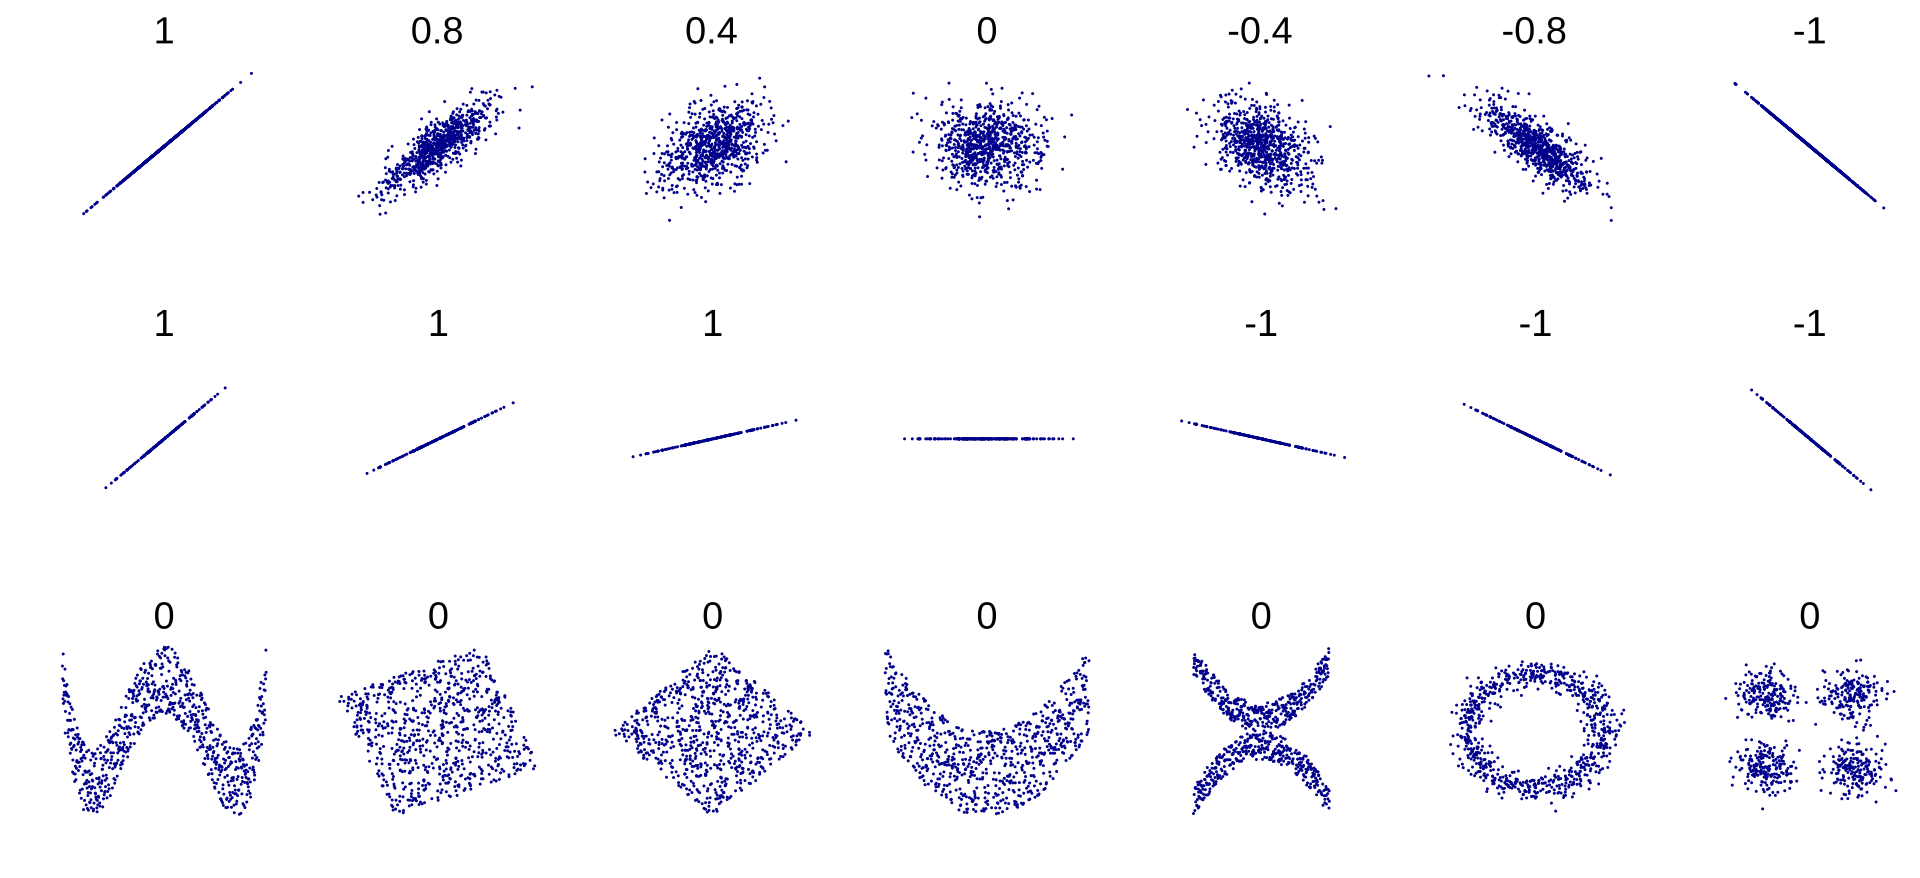
\includegraphics[width=0.9\linewidth]{chapters/chapter 10/correlation.png}
\end{figure}


\section{Բաշխումներ}

Եթե որոնեք, թե ինչպես են բաշխված այս կամ այն երկրում մարդկանց աշխատավարձերը, հասակները, քաշերը և այլն, կնկատեք մի տար\-օրի\-նակ նմանություն դրանց \href{https://images.app.goo.gl/viKPLRbQKCsQfbhLA}{խտության գրաֆիկներում}․ կարծես բոլորը մո\-տա\-վո\-րա\-պես նույն գրաֆիկը լինեն՝ ինչ-որ չափով ձգված, սեղմված կամ տեղա\-շարժ\-ված։ Առանց պատ\-ճառ\-նե\-րի մեջ խորանալու նկատենք, որ այսպիսի նմա\-նու\-թյուն\-ներ հանդիպում են ամե\-նա\-տար\-բեր պրոցեսների արդյունքում առա\-ջա\-ցող պատա\-հա\-կան մեծու\-թյուն\-ների բաշխումներում։ Ուրեմն եթե 
% այդ տարբեր, բայց միմյանց նման բաշխումներին տանք մեկ միասնական անուն ու 
ընդհանուր դեպքում այդ պատահական մեծություններից մեկի բաշխումը հետազոտենք, ապա հետազոտած կլինենք նաև նույն կաղապարով/ֆորմայով ստացված մյուս բաշխումները։

Իրականում մենք մի անգամ նման բան արել ենք, երբ
\begin{itemize}
\item $[0, 10]$ հատվածում ընտրում ենք պատահական կետ
\item $12$:$00$-$13$:$00$ պատահական պահի գալիս ենք կանգառ
\item գեներացնում ենք պատահական թիվ $(-1, 1)$ միջակայքում
\item $\dots$
\end{itemize}
այս բոլոր պատահական մեծություններին տվեցինք մեկ ընդհանրական անուն՝\marginnote{իհարկե համարելով, որ ցանկացած տե\-ղա\-մասում գտնվող արժեքներն ունեն նույն հավանականությունը} ասելով, որ դրանք \textit{հավասարաչափ բաշխում} ունեն, և գտնելով $\operatorname{U}(a, b)$ բաշխումով ցանկացած պատահական մեծության {\rm CDF}-ն ու {\rm PDF}-ը (որոնք ազատ կարող ենք օգտագործել նշված բոլոր մասնավոր օրինակների համար)։  

Եկեք այժմ նույն կերպ դիտարկենք մի քանի հիմնական բաշխումներ (անգիր անել պետք չէ), որոնք հանդիպում են տարբեր պրոցեսներում։ Սկսենք դիսկրետ բաշխումներից։

\begin{description}
\item[Բեռնուլիի բաշխում․] 
Դիտարկենք հետևյալ իրավիճակները՝
\begin{itemize}
    \item նետում ենք մետաղադրամ
    \item մտնում ենք վարորդական իրավունքի քննության
    \item կրակում ենք թիրախին
    \item ջնջում ենք լոտո
\end{itemize}
Դրանցից յուրաքանչյուրում կա երկու հնարավոր տարբերակ՝ գիր կամ ղուշ, անցնել կամ կտրվել, դիպչել կամ ոչ, շահել կամ չշահել, և այլն։ Այսպիսի փորձերը կանվանենք \textit{Բեռնուլիի փորձեր,} իսկ երկու հնարավոր արժեք ընդունող (մեկը՝ $p$, մյուսը՝ $1-p$ հավանականությամբ) ցանկացած պատահական մեծության մասին կասենք, որ այն ունի Բեռնուլիի բաշխում՝
\[
X \sim \operatorname{Bernoulli}(p)
\]
Հեշտությամբ կարող ենք հաշվել, որ այս դեպքում
\[
\E[X] = p, \qquad \Var[X] = p(1-p)
\]

\item[Երկրաչափական բաշխում․]
Իսկ ի՞նչ, եթե որոշենք լոտոներ ջնջել այնքան, մինչև վերջապես շահենք (կամ ավելի խելացի միտք՝ քննություն տանք այնքան, մինչև վերջապես անցնենք)։ Քանի՞ անգամ կպահանջվի մինչև առաջին անգամ շահելը/անցնելը, կամ որ նույնն է՝ քանի՞ անգամ պետք է կրկնենք շահելու $p$ հավանականություն ունեցող Բեռնուլիի փորձը, մինչև առաջին անգամ շահենք։

Նշանակենք այդ փորձերի քանակը $X$-ով և գտնենք $p_X(k)$-ն։ Նախ՝ հավանականությունը, որ $X=1$, այսինքն՝ որ հենց առաջին փորձից կստացվի անցնել քննությունը, $p$ է։ 

Իսկ որ $X=2$, այսինքն՝ առաջին անգամը կկտրվենք, իսկ երկ\-րորդին արդեն կանցնենք, հավասար է
\[
\PP[X = 2] = \underbrace{\color{myred}(1 - p)}_{\substack{\text{$1$-ինը}\\\text{կտրվենք}}} \ \cdot \underbrace{\color{mygreen}p}_{\substack{\text{$2$-րդը}\\\text{անցնենք}}}
\]
Հավանականությունը, որ $X=3$՝
\[
\PP[X = 3] = \underbrace{\color{myred}(1 - p)}_{\substack{\text{$1$-ինը}\\\text{կտրվենք}}} \ \cdot \ \underbrace{\color{myred}(1 - p)}_{\substack{\text{$2$-րդը}\\\text{կտրվենք}}} \ \cdot \underbrace{\color{mygreen}p}_{\substack{\text{$3$-րդը}\\\text{անցնենք}}}
\]

\begin{marginfigure}
    \centering
    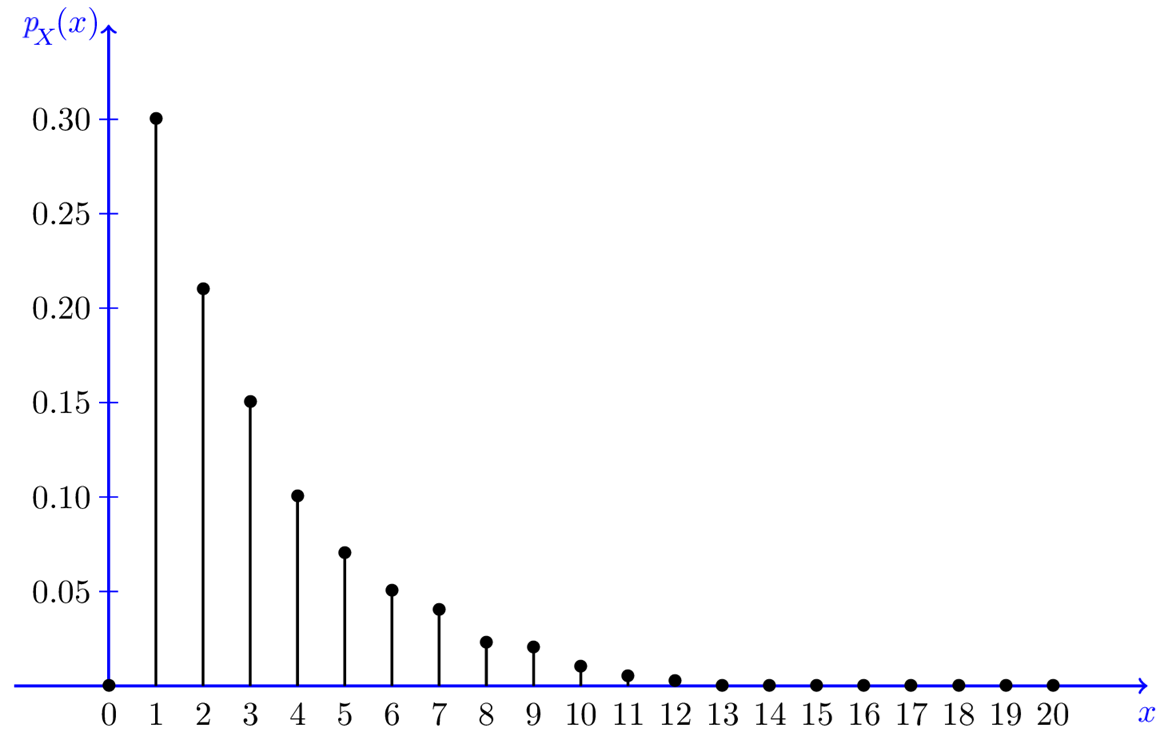
\includegraphics[width=\linewidth]{chapters/chapter 10/geometric.png}
    \caption*{$X$-ի {\rm PMF}-ը, երբ $p=0.3$}
\end{marginfigure}

Եվ այդպես շարունակ՝
\[
\PP[X = k] = {\color{myred}(1 - p)} \cdot {\color{myred}(1 - p)} \cdot \ldots \cdot {\color{myred}(1 - p)} \cdot {\color{mygreen}p} 
= (1 - p)^{k-1} \cdot p
\]
այսինքն $k$-ն $1$-ով մեծացնելիս հավանականությունը բազմա\-պատկ\-վում է $(1-p)$-ով՝ դառնալով երկրաչափական պրոգրեսիա։ Նման դեպքերում կասենք, որ $X$-ն ունի երկրաչափական բաշխում՝
\[
X \sim \operatorname{G}(p)
\]
և կունենանք
\[
\E[X] = \frac{1}{p}, \qquad \Var[X] = \frac{1 - p}{p^2}
\]

\question{Կարո՞ղ եք ապացուցել, որ եթե արդեն իսկ $100$ անգամ \newline ջնջել ու չեք շահել, դա Ձեզ ավելի մոտ չի դարձնում շահելուն։}
Այլ կերպ ասած՝
\[
\PP[X > m + n \mid X > m] = \PP[X > n]
\]
Այս հատկության մասին ասում են, որ երկրաչափական բաշխումը \textit{հիշողություն չունի։}

\item[Բինոմական բաշխում․]
Մյուս կողմից՝ եթե իրար հետևից հանձնեք մի քանի քննություն, ասենք՝ $n$ հատ, և ամեն մեկում ունենաք անցնելու նույն $p$ հավանականությունը, կարող եք հարցնել՝ որքա՞ն է հավանական, որ կանցնեք բոլոր $n$ քննությունները, կամ քննությունների կեսը, կամ $3$ հատը, և այլն։

Եթե $X$-ով նշանակենք, թե այդ $n$ Բեռնուլիի փորձերից քանի՞սն են հաջողությամբ պսակվել, կունենանք՝\marginnote[*+4]{$C_n^k$-ն կարդացվում է «զուգորդություն $n$-ից $k$-ական», նշանակվում է նաև $\displaystyle \binom{n}{k}$}
\[
\PP[X = k] \ = \underbrace{C_n^k}_{\substack{\text{$n$ հատից $k$ հատ}\\\text{ընտրելու ձևերը}}} \cdot \ \overbrace{p^k}^{\substack{\text{$k$ անգամ}\\\text{կանցնենք}}} \cdot \ \underbrace{(1 - p)^{n-k}}_{\substack{\text{$n-k$ անգամ}\\\text{կկտրվենք}}}
\]
որտեղ $C_n^k = \dfrac{n!}{k!\cdot(n-k)!}$: 

\begin{marginfigure}
    \centering
    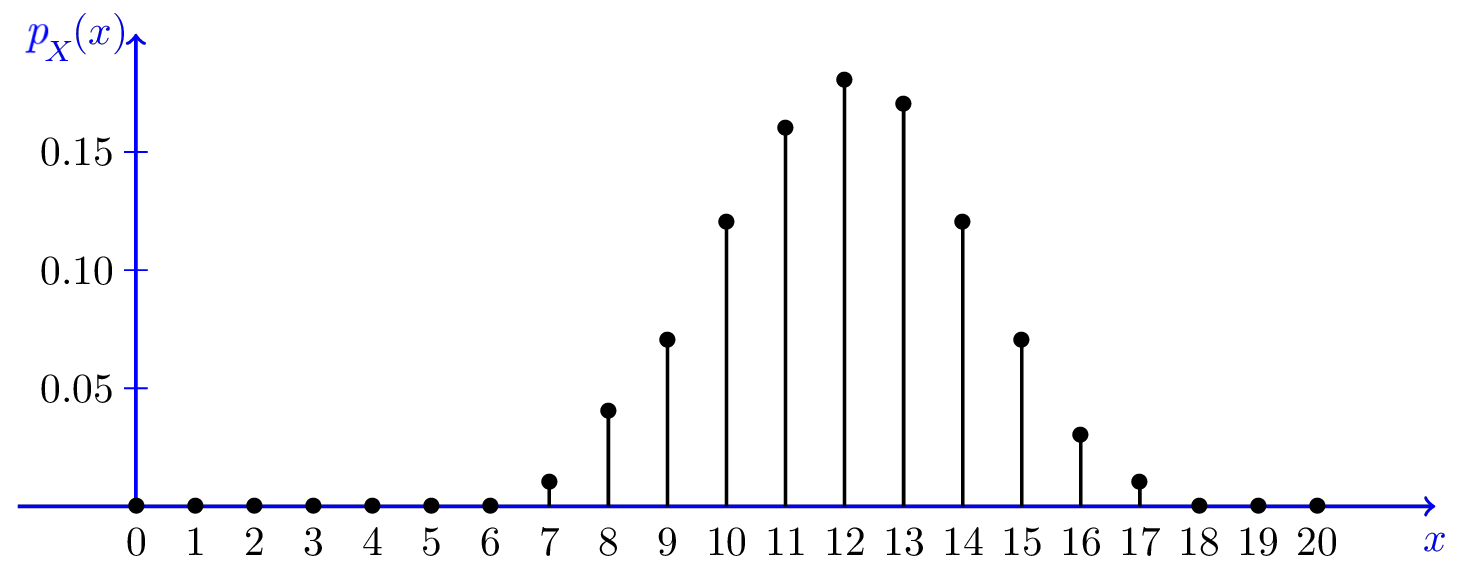
\includegraphics[width=\linewidth]{chapters/chapter 10/binomial.png}
    \caption*{$X$-ի {\rm PMF}-ը, երբ $n=20$, $p=0.6$}
\end{marginfigure}

Այս բանաձևերը պետք չէ անգիր անել․ դրանց շատ գեղեցիկ բացատրությունն ու դուրս բերումը կարող եք գտնել \href{https://www.youtu.be/8idr1WZ1A7Q}{այստեղ} կամ \href{https://www.youtu.be/6YzrVUVO9M0}{այստեղ}։ Այս դեպքում կասենք, որ $X$-ն ունի բինոմական բաշխում՝
\[
X \sim \operatorname{B}(n, p)
\]
և կունենանք՝
\[
\E[X] = np, \qquad \Var[X] = np(1-p) 
\]

\item[Պուասոնի բաշխում․] 
Եկեք ոչ թե իրար հետևից ինչ-որ փորձեր կրկնենք, այլ պարզապես հաշվենք, թե
\begin{itemize}
    \item քանի հաճախորդ մտավ $13$:$00$-$14$:$00$ հատվածում
    \item քանի ավտովթար եղավ օրվա ընթացքում
    \item քանի զանգ եկավ սխալ համարից
    \item քանի գոլ եղավ խաղի ժամանակ
    \item քանի ավտոբուս անցավ կանգառով $1$ ժամում 
\end{itemize}
այսինքն՝ հաշվենք, թե ամեն անգամը նախորդից անկախ տեղի ունեցող մի որևէ երևույթից քանի անգամ արձանագրվեց ֆիքսված ժամանակամիջոցում։ Ստացված քանակը (ենթադրենք՝ խանութ մտած այցելուների) նշանակենք $X$-ով։

Եթե ասենք՝ նախորդ շաբաթվա տվյալների հիման վրա իմանանք, թե միջինում\marginnote{այսինքն՝ վայրկյանը մեկ նա\-յում ենք՝ մարդ մտա՞վ, թե՞ ոչ․ \[X \sim \operatorname{B}\left(3600, \dfrac{\lambda}{3600}\right)\] իսկ սրա {\rm PMF}-ը  $\approx \dfrac{\lambda^k}{k!} \cdot e^{-\lambda}$ է} $13$:$00$-ից $14$:$00$-ը քանի հոգի է մտնում խանութ (օրինակ՝ միջինում $\lambda=20$ հոգի), ապա կունենանք՝
\[
\PP[X = k] = \frac{\lambda^k}{k!} \cdot e^{-\lambda}
\]
և կասենք, որ $X$-ն ունի Պուասոնի բաշխում՝
\[
X \sim \operatorname{Poisson}(\lambda)
\]
\begin{marginfigure}
    \centering
    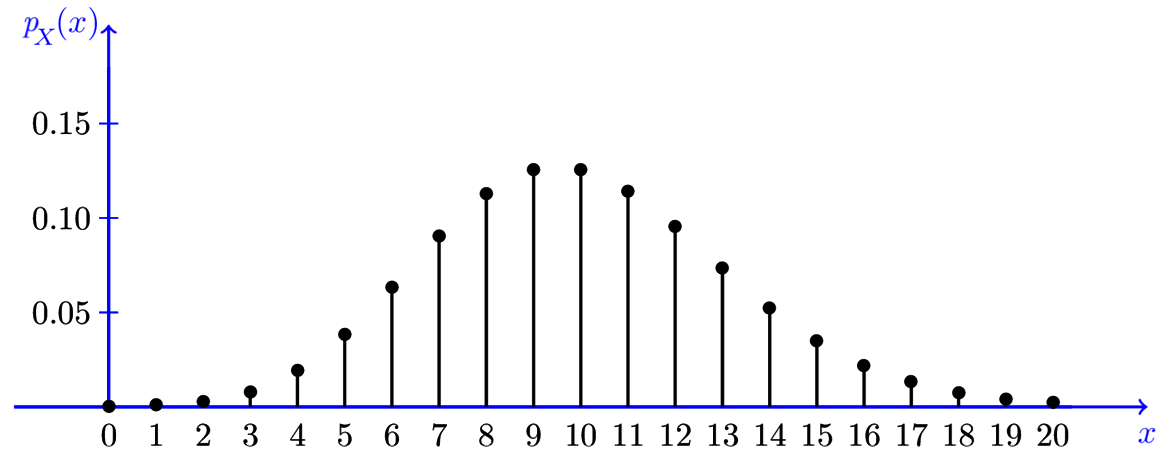
\includegraphics[width=\linewidth]{chapters/chapter 10/poisson.png}
    \caption*{$X$-ի {\rm PMF}-ը, երբ $\lambda=10$}
\end{marginfigure}
\question{Ճանաչո՞ւմ եք այս թվերը։}

Այս դեպքում մաթսպասումն ու վարիացիան համընկնում են՝
\[
\E[X] = \lambda, \qquad \Var[X] = \lambda
\]
\end{description}

Եվ այդպես շարունակ։ Կան \href{https://en.wikipedia.org/wiki/List_of_probability_distributions}{բազմաթիվ} այլ օգտակար բաշխումներ, որոնք հանդիպում են տարբեր իրավիճակներում, բայց դրանք անգիր հիշելու կամ բոլորը իմանալու կարիք չկա։

Անցնենք անընդհատ բաշխումներին։

\begin{description}
\item[Հավասարաչափ բաշխում․]
Անձամբ ճանաչում ենք։ Ավելացնենք միայն, որ եթե $X \sim \operatorname{U}(a, b)$, ապա
\[
\E[X] = \frac{a + b}{2}, \qquad \Var[X] = \frac{(b - a)^2}{12}
\]

\item[Ցուցչային {\normalfont (էքսպոնենցիալ)} բաշխում․]
Սա մեր երկրաչափական բաշխ\-ման անընդհատ անալոգն է։ Պատկերացրեք՝ հենց նոր ան\-ցավ ավտոբուսը, և կանգնած սպասում եք, թե քանի րոպեից կգա հաջորդը։ Այդ $X$ ժամանակահատվածը, \marginnote{կարող ենք համարել, որ աչքերը բացում ենք, նայում՝ ավտոբուս կա, թե ոչ, փա\-կում, \href{https://youtu.be/TZTjr-DN9xY?si=vfGqcFPmMgqd-bqp&t=1794}{ապա նորից}, այնքան մինչև գա} այսինքն՝ թե որքան է պետք սպասել, մինչև ինչ-որ երևույթ նորից տեղի ունենա, ունի ցուցչային բաշխում՝
\[
X \sim \operatorname{Exp}(\lambda)
\]
որտեղ $\lambda$-ով նշանակում ենք, թե միջինում որքան ժամանակը մեկ է գալիս ավտոբուսը։

\begin{marginfigure}
    \centering
    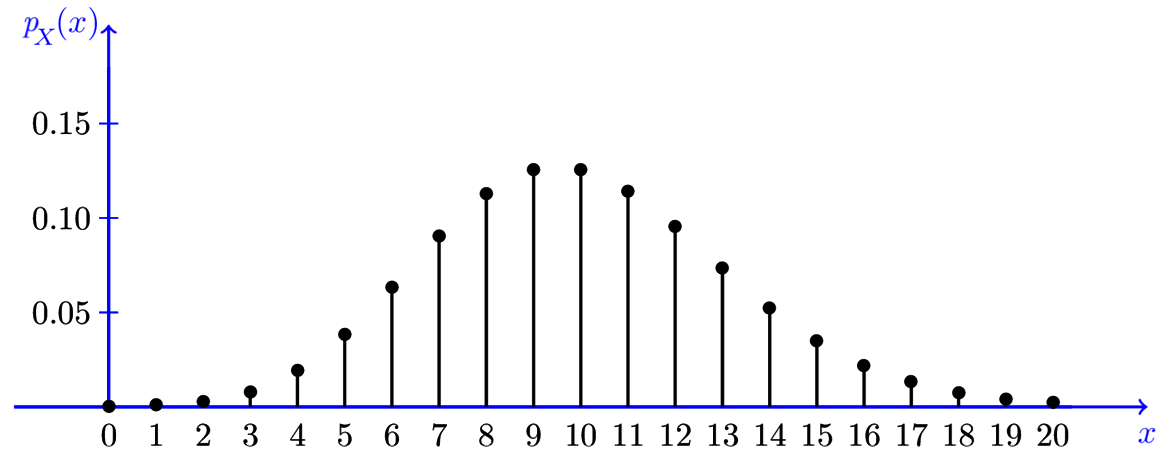
\includegraphics[width=\linewidth]{chapters/chapter 10/poisson.png}
    \caption*{$X$-ի {\rm PDF}-ը տարբեր $\lambda$-ների դեպքում}
\end{marginfigure}

$X$-ի խտության ֆունկցիան կունենա հետևյալ տեսքը՝
\[
f_X(x) = \begin{cases}
    \lambda e^{-\lambda x} & \text{եթե } x \ge 0 \\
    0 & \text{եթե } x < 0
\end{cases}
\]
իսկ մաթսպասումն ու վարիացիան կլինեն
\[
\E[X] = \frac{1}{\lambda}, \qquad \Var[X] = \frac{1}{\lambda^2}
\]
Ինչպես երկրաչափական, այնպես էլ ցուցչային բաշխումը հիշո\-ղու\-թյուն չունի՝
\[
\PP[X > a + b \mid X > b] = \PP[X > a]
\]
այսինքն՝ եթե արդեն իսկ $b$ րոպե սպասել ենք, բայց ավտոբուսը դեռ չի եկել, ապա հավանականությունը, որ այն կգա ևս $a$ րոպե անց, նույնն է, ինչ եթե սկզբի $b$ րոպեն սպասած չլինեինք։ Ավտոբուսը չգիտի՝ իրեն սպասել ենք, թե ոչ․ մեր սպասելուց ոչինչ չի փոխվում։

\item[Նորմալ {\normalfont (գաուսյան)} բաշխում․]
Ինչ-որ իմաստով՝ սա ամենակարևոր բաշխումն է։ Պատկերացրեք՝ եթե
\begin{itemize}
    \item նետենք $100$ հատ զառ
    \item չափենք պատահական $1000$ հոգու հասակ
    \item հաշվենք $500$ պատահական բառերի տառեր
    \item իրար վրա լցնենք \href{https://youtu.be/UCmPmkHqHXk}{տարերային շարժվող գնդիկներ}
\end{itemize}
ու նայենք, թե ինչ $X$ թիվ ենք ստանում \marginnote{այսինքն՝ նույն բաշխումը ունեցող մեծ թվով պատահական մեծությունների միջինը} \textbf{միջինում,} ապա
այդ $X$-ը կլինի պատահական մեծություն (ընդ որում՝ անընդհատ), և նրա խտության ֆունկցիան կունենա հետևյալ տեսքը՝
\[
f_X(x) = \frac{1}{\sqrt{2\pi \sigma^2}}e^{-\dfrac{(x - \mu)^2}{2\sigma^2}}
\]

\begin{figure}[b]
    \centering
    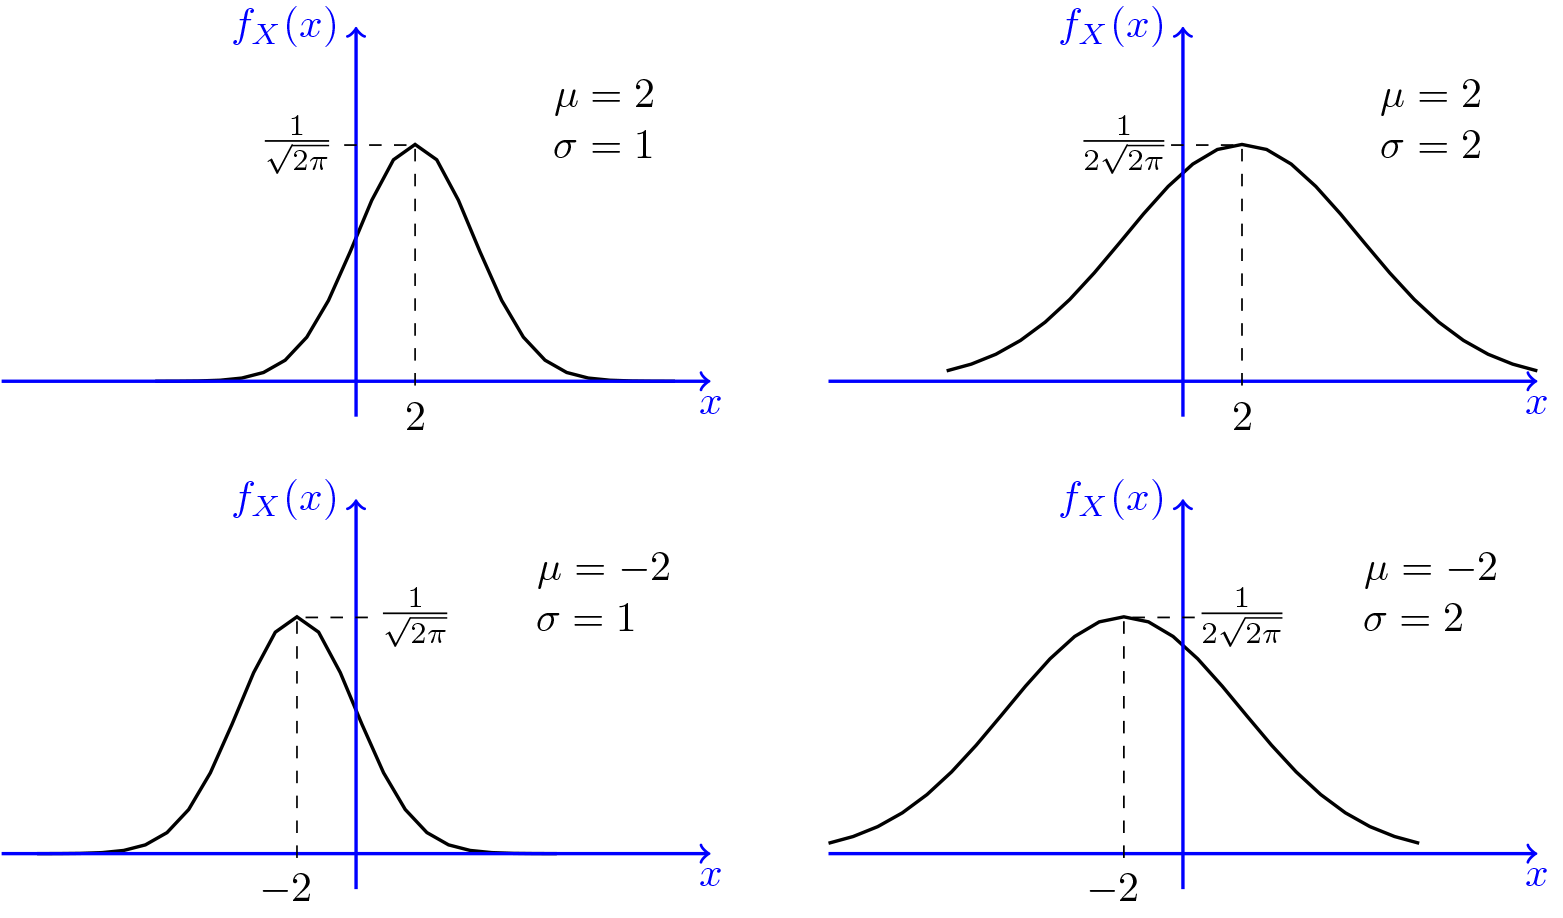
\includegraphics[width=0.85\linewidth]{chapters/chapter 10/normal.png}
\end{figure}

որտեղ $\mu$-ն ու $\sigma^2$-ն նրա մաթսպասումն ու վարիացիան են՝
\[
\E[X] = \mu, \qquad \Var[X] = \sigma^2
\]

\question{Ինչպե՞ս կփոխվի $f_X$-ի գրաֆիկը, եթե $\mu$-ն մեծացնենք \newline $7$-ով, իսկ $\sigma$-ն բազմապատկենք $2$-ով:}

Թե ինչու է սա ճիշտ, և ինչու է արդյունքում ստացվում այսպիսի զանգակաձև կոր, բխում է «կենտրոնական սահմանային թեորեմ» կոչվող մի հետաքրքիր փաստից, որը մենք կշրջանցենք և պարզապես կասենք, որ $X$-ն ունի նորմալ կամ գաուսյան բաշխում՝
\[
X \sim \operatorname{N}(\mu, \sigma^2)
\]
Մասնավորապես ${X \sim \operatorname{N}(0, 1)}$ դեպքում կասենք, որ $X$-ն ունի \textit{ստան\-դարտ} նորմալ բաշխում։ Նորմալ բաշխում ունեցող ցան\-կա\-ցած $X$-ից կարող ենք իր $\mu$ միջինը հանելով ու $\dfrac{1}{\sigma}$-ով բազ\-մա\-պատ\-կելով՝ այն դարձնել ստանդարտ նորմալ։
\end{description}


\bigskip 

\begin{theory}
.
\begin{itemize}
\item կարդալ [{\rm Blitzstein-Hwang}], 137-143, 156-159, 200, կամ [{\rm Grimmett-Welsh}], 30-32, 73-74 էջերը (մաթսպասում, վարիացիա)
\item տեսնել \href{https://www.countbayesie.com/blog/2015/2/20/random-variables-and-expectation}{մաթսպասումն} ու \href{https://www.countbayesie.com/blog/2015/2/21/variance-co-variance-and-correlation}{վարիացիան} կոնկրետ օրինակով 
\item կարդալ [{\rm Blitzstein-Hwang}], 300-304, կամ [{\rm Grimmett-Welsh}], 113-117 էջերը (կովարիացիա, կոռելացիա)
\item տեսնել, թե \href{https://dlsun.github.io/skis/discrete/named-distributions.html}{դիսկրետ} և \href{https://dlsun.github.io/skis/continuous/named-distributions.html}{անընդհատ} բաշխումներից որը երբ է հանդիպում
\item ըստ ցանկության՝ կարդալ բաշխումների մասին [{\rm Blitzstein-Hwang}], 100-103 (Բեռնուլի, բինոմական), 161-164 (Պուասոն), 201-202 (հավասարաչափ), 211-212 (նորմալ), 217-219 (ցուց\-չա\-յին) էջերը
\item ըստ ցանկության՝ դիտել կենտրոնական սահմանային թեո\-րեմի մասին \href{https://youtu.be/zeJD6dqJ5lo}{տեսանյութ} {\rm 3b1b}-ից
\end{itemize}
\end{theory}

\newpage

\section{Խնդիրներ}


\begin{problem}
Հնարամիտ ուստա Վարդանն առաջարկում է խաղալ հետևյալ խաղը։ Նետում եք զառը, և
\begin{itemize}
    \item եթե ընկնում է $1$, ուստա Վարդանը Ձեզ տալիս է $2\,500$ դրամ
    \item եթե ընկնում է $2$, տալիս է $5000$ դրամ
    \item եթե ընկնում է $3$, ոչ ոք ոչինչ չի տալիս
    \item եթե ընկնում է $4$ կամ $5$, Դուք եք $10\,000$ դրամ տալիս ուստա Վար\-դանին
    \item եթե ընկնում է $6$, տալիս եք $15\,000$ դրամ
\end{itemize}
Ցանկանո՞ւմ եք խաղալ այս խաղը։ Ինչո՞ւ։
\end{problem}


\begin{problem}
Վահեն զառի 
\includegraphics[height=1.6ex]{chapters/chapter 8/dice/4.png} կողմի վրա նկարեց ևս մի կետ՝ դարձնելով այն 
\includegraphics[height=1.6ex]{chapters/chapter 8/dice/5.png}, իսկ 
\includegraphics[height=1.6ex]{chapters/chapter 8/dice/1.png} կողմի վրա ավելացրեց երկու կետ՝ դարձնելով այն 
\includegraphics[height=1.6ex]{chapters/chapter 8/dice/3.png}։ 

Որքա՞ն է հավանականությունը, որ զառը նետելիս կընկնի $4$-ից մեծ թիվ։ Որքա՞ն են զառի մաթսպասումն ու վարիացիան։
\end{problem}


\begin{problem}
$52$ հատ խաղաթղթերից պատահականորեն քաշում եք մեկը։ Եթե
\begin{itemize}
    \item հանեցիք սիրտ, շահում եք $10\,000$ դրամ
    \item սիրտ չէ, բայց վրան մարդ է պատկերված, շահում եք $8\,000$ դրամ
    \item մնացած դեպքերում կորցնում եք $6\,000$ դրամ
\end{itemize}

Ձեռնտո՞ւ է խաղալ այս խաղը։ Միջինում որքա՞ն կշահեք/կկորցնեք ամեն խաղի արդյունքում։
\end{problem}


\begin{problem}
$X$ պատահական մեծության խտության ֆունկցիան է՝
\[
f_X(x) = \begin{cases}
    \frac{3}{x^4} & \text{եթե } x \ge 1 \\
    0 & \text{մնացած դեպքերում}
\end{cases}
\]
Գտեք $\E[X]$-ն ու $\Var[X]$-ը։
\end{problem}


\begin{problem}
$X$ պատահական մեծության խտության ֆունկցիան է՝
\[
f_X(x) = \begin{cases}
   2x & \text{եթե } 0 \le x \le 1 \\
   0 & \text{մնացած դեպքերում} 
\end{cases}
\]
Որքա՞ն են հետևյալ պատահական մեծություններից յուրաքանչյուրի մաթսպասումն ու վարիացիան․
\begin{enumerate}[label={\alph*}․]
\item $X$
\item $2X$
\item $2X + 7$
\item $(2X + 7)\cdot Y$
\end{enumerate}
որտեղ $Y$-ը պատահական նետված զառի թիվն է։
\end{problem}


\begin{problem}
$X$-ն ու $Y$-ը հավասարաչափ բաշխված անկախ պա\-տա\-հա\-կան մեծություններ են, ընդ որում՝
\[
X \sim \operatorname{U}(0, 2), 
\qquad
Y \sim \operatorname{U}(4, 10)
\]

\newpage

Կարո՞ղ եք գտնել
\begin{enumerate}[label={\alph*}․]
\item $X + Y$-ի մաթսպասումը
\item $XY$-ի մաթսպասումը
\item $X + Y$-ի խտության ֆունկցիան
\end{enumerate}

Ի՞նչ բաշխում ունի $X + Y$ պատահական մեծությունը։ Իսկ $XY$-ը՞։
\end{problem}
